%%%%%%%%%%%%%%%%%%%%%%%%%%%%%%%%%%%%%%%%%%%%%%%%%%%%%%%%%%%%%%%%%%%%%%%%%%%%%%%
\section{Context \& Background}
%%%%%%%%%%%%%%%%%%%%%%%%%%%%%%%%%%%%%%%%%%%%%%%%%%%%%%%%%%%%%%%%%%%%%%%%%%%%%%%


%%%%%%%%%%%%%%%%%%%%%%%%%%%%%%%%%%%%%%%%%%%%%%%%%%%%%%%%%%%%%%%%%%%%%%%%%%%%%%%
\begin{frame}{Supervised Learning Algorithms}
%%%%%%%%%%%%%%%%%%%%%%%%%%%%%%%%%%%%%%%%%%%%%%%%%%%%%%%%%%%%%%%%%%%%%%%%%%%%%%%
  \begin{figure}
    \begin{minipage}[!ht]{0.42\textwidth}
      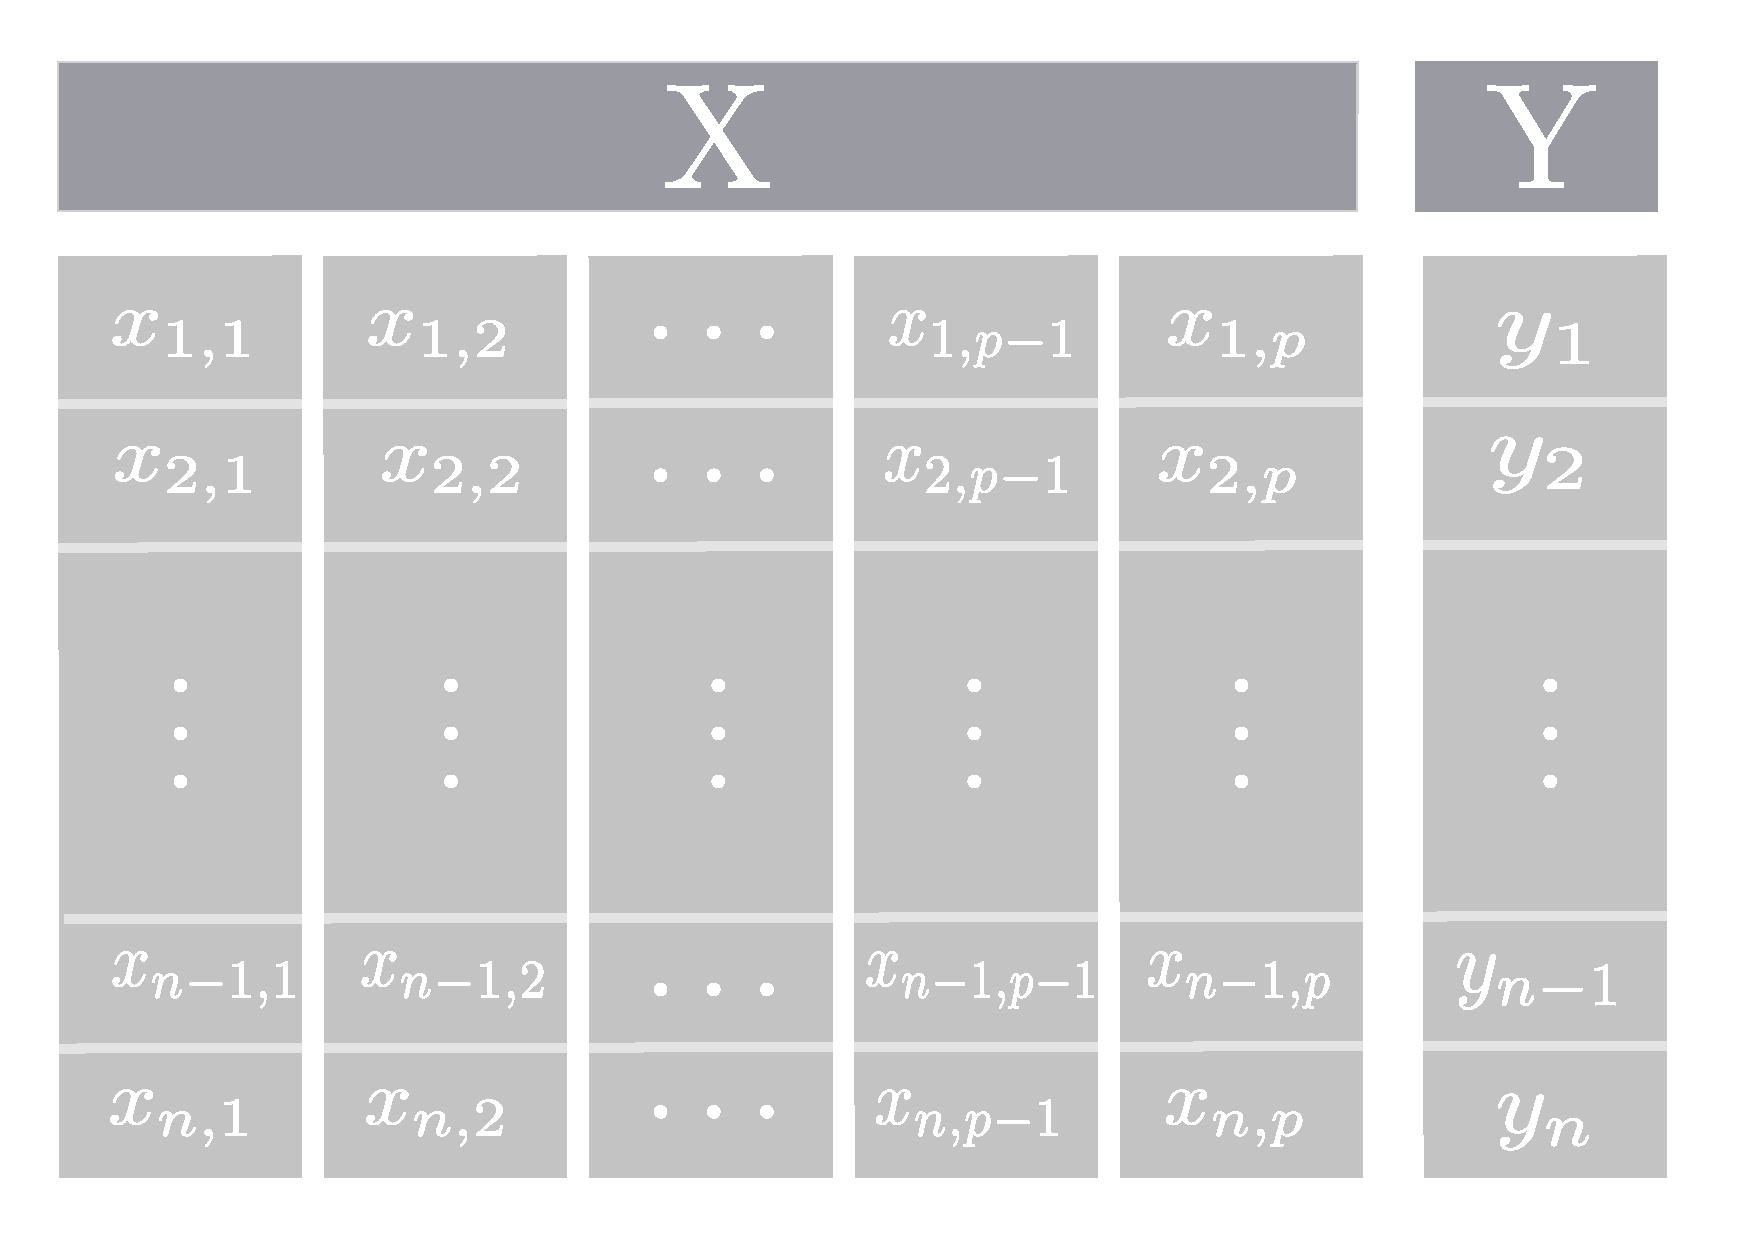
\includegraphics[width=\textwidth]{images/TableauDonneeApprentissage.pdf}
    \end{minipage} \hspace{0.3cm}
    \begin{minipage}[!ht]{0.52\textwidth}
      Given a set of $n$ \textbf{training examples} $\left\{ (\xvec_1, y_1),\dots,(\xvec_n, y_n) \right\}$ where $\xvec_i$ is the feature vector of the $i^{th}$ example, and $y_i$ is the corresponding label. \\
      \textbf{Assumption:} there is a function $f$ matching any feature vector to its label.
   \end{minipage}
  \end{figure}
    The goal of a \textbf{learning algorithm} is to approximate $f$ by a parameterized function $f_\theta$.
    In order to measure how well the function fits, \textbf{a loss function} $\mathcal{L}: \mathcal{Y} \times \mathcal{Y} \rightarrow \Rbb^{+}$ is defined.
    The standard method to learn the set of parameters $\theta$ is the \textbf{empirical risk minimization (ERM)}:
  \begin{equation*}
    \hat{\theta}_{ERM} \triangleq \argmin_{\theta} \frac{1}{n} \sum_{i=1}^{n} \mathcal{L} (f_{\theta} (\xvec_i), y_i )
  \end{equation*}
\end{frame}



%%%%%%%%%%%%%%%%%%%%%%%%%%%%%%%%%%%%%%%%%%%%%%%%%%%%%%%%%%%%%%%%%%%%%%%%%%%%%%%
\begin{frame}{Deep neural networks}
%%%%%%%%%%%%%%%%%%%%%%%%%%%%%%%%%%%%%%%%%%%%%%%%%%%%%%%%%%%%%%%%%%%%%%%%%%%%%%%

  Neural Neural can be analytically described as a composition of linear functions interlaced with non-linear functions:
  \begin{block}{Neural Network}
      A neural network of $\ell$ layers is defined as follows:
      \begin{equation*}
	\mathcal{N}_\theta(\xvec) = \phi_{\Wmat_\ell,\bvec_\ell} \circ \rho \circ \phi_{\Wmat_{\ell-1}, \bvec_{\ell-1}} \circ \rho \circ \cdots \circ \rho \circ \phi_{\Wmat_1, \bvec_1}(\xvec)
      \end{equation*}
      where for any $i$, $\phi_{\Wmat_i,\bvec_i} \triangleq \xvec \mapsto \Wmat_i \xvec + \bvec_i$, $\xvec_i \in \Rbb^n$, $\bvec_i \in \Rbb^m$, $\Wmat_i \in \Rbb^{m \times n}$, $\rho$ some non linear functions and $\theta$ corresponds to the set of all parameters.
  \end{block}

  \begin{block}{Evaluation of Neural Networks}
    \begin{itemize}
      \item[$\bullet$] Classical evaluation with accuracy
      \item[$\bullet$] Robust evaluation against adversarial attacks
    \end{itemize}
  \end{block}

\end{frame}


%%%%%%%%%%%%%%%%%%%%%%%%%%%%%%%%%%%%%%%%%%%%%%%%%%%%%%%%%%%%%%%%%%%%%%%%%%%%%%%
\begin{frame}{Adversarial Attacks}
%%%%%%%%%%%%%%%%%%%%%%%%%%%%%%%%%%%%%%%%%%%%%%%%%%%%%%%%%%%%%%%%%%%%%%%%%%%%%%%
  An \textbf{adversarial attack} refers to a small, imperceptible change of an input maliciously designed to fool the result of a machine learning algorithm. 
  \begin{center}
    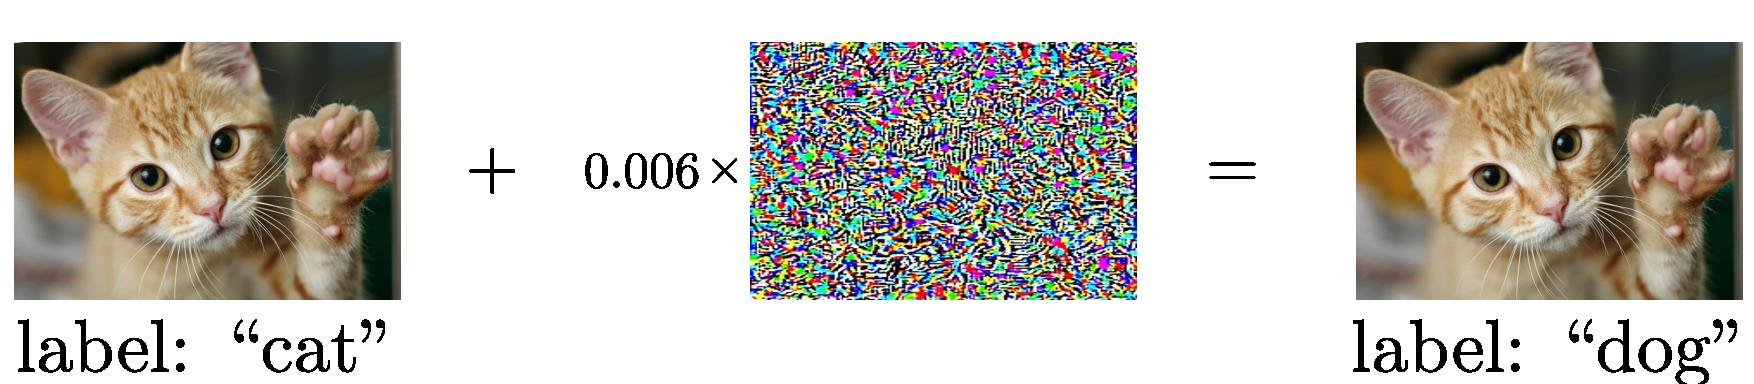
\includegraphics[width=\textwidth]{images/ExampleAdversarialCatDog.pdf}
  \end{center}
  Since the seminal work of \cite{Szegedy2013IntriguingPO}, numerous attack methods have been designed:
  \begin{itemize}
    \item[$\bullet$] \textbf{PGD} \cite{madry2018towards}
    \item[$\bullet$] \textbf{C\&W} \cite{carlini2017towards}
  \end{itemize}

\end{frame}


% %%%%%%%%%%%%%%%%%%%%%%%%%%%%%%%%%%%%%%%%%%%%%%%%%%%%%%%%%%%%%%%%%%%%%%%%%%%%%%%
% \begin{frame}{Adversarial Attacks}
% %%%%%%%%%%%%%%%%%%%%%%%%%%%%%%%%%%%%%%%%%%%%%%%%%%%%%%%%%%%%%%%%%%%%%%%%%%%%%%%
%
%   Given an input-output pair $(\xvec, y) \sim \mathcal{D}$, an \textbf{adversarial attack} is a procedure that produces a small perturbation $\mathbf{\tau} \in \mathcal{X}$ such that $\mathcal{N}_\theta(\xvec + \mathbf{\tau}) \neq y$.
%
%   Existing attacks can adopt one of the two following strategies:
%   \begin{itemize}
%     \item[1.] maximizing the loss $\mathcal{L}(\mathcal{N}_\theta(\xvec + \tau), y)$ under some constraint on $\norm{\tau}_p$;
%     \item[2.] minimizing $\norm{\tau}_p$ under some constraint on the loss $\mathcal{L}(\mathcal{N}_\theta(\xvec + \tau), y)$;
%   \end{itemize}
%
%   In the following, we will use:
%   \begin{itemize}
%     \item Strategy 1: \textbf{PGD}-$\ell_\infty$ attack (\cite{madry2018towards})
%     \item Strategy 2: \textbf{C\&W}-$\ell_2$ attack (\citet{carlini2017towards})
%   \end{itemize}
%
% \end{frame}



%%%%%%%%%%%%%%%%%%%%%%%%%%%%%%%%%%%%%%%%%%%%%%%%%%%%%%%%%%%%%%%%%%%%%%%%%%%%%%%
\begin{frame}{Limits of Large Neural Networks}
%%%%%%%%%%%%%%%%%%%%%%%%%%%%%%%%%%%%%%%%%%%%%%%%%%%%%%%%%%%%%%%%%%%%%%%%%%%%%%%

  Fully-Connected Neural Networks (neural networks defined with dense matrices) can have a \emph{very large number of parameters}.

  $\Rightarrow$ With MNIST dataset (\cite{lecun1998gradient}), a two-layers Fully-Connected neural network will have more than $\mathbf{6 \times 10^5}$ \textbf{parameters}.

  \vspace{0.5cm}

  \begin{block}{Limits of Large Neural Networks}
    \begin{itemize}
      \small
      \item[$\bullet$] They are hard to train
      \item[$\bullet$] They are subject to overfitting: they don't generalize well
      \item[$\bullet$] They are computationally expensive 
    \end{itemize}
  \end{block}
  
  $\Rightarrow$ To overcome these limitations, researchers have devised neural networks with \textbf{structured linear operations} in order to reduce the number of parameters needed.

\end{frame}



%%%%%%%%%%%%%%%%%%%%%%%%%%%%%%%%%%%%%%%%%%%%%%%%%%%%%%%%%%%%%%%%%%%%%%%%%%%%%%%
\begin{frame}{Structured matrices for Deep Neural Networks}
%%%%%%%%%%%%%%%%%%%%%%%%%%%%%%%%%%%%%%%%%%%%%%%%%%%%%%%%%%%%%%%%%%%%%%%%%%%%%%%

  A $n \times n$ structured matrix can be represented with less than $n^2$ parameters. In addition to offering a more compact representation, the structure of certain matrices can be leveraged to obtain better algorithms for matrix-vector product.

  \begin{figure}[ht]
     \centering
     \begin{subfigure}[t]{2.2cm}
	 \centering
	 \begin{equation*}
	   \begin{pmatrix}
	      a &   &   &   \\
		& b &   &   \\
		&   & c &   \\
		&   &   & d
	   \end{pmatrix}
	 \end{equation*}
	 \caption*{diagonal}
     \end{subfigure}
     \begin{subfigure}[t]{2.2cm}
	 \centering
	 \begin{equation*}
	    \begin{pmatrix}
	      a & b & c & d \\
	      e & a & b & c \\
	      f & e & a & b \\
	      d & f & e & a
	    \end{pmatrix}
	 \end{equation*}
	 \caption*{Toeplitz}
     \end{subfigure}
     \begin{subfigure}[t]{2.8cm}
	 \centering
	 \begin{equation*}
	    \begin{pmatrix}
	      ae & af & ag & ah \\
	      be & bf & bg & bh \\
	      ce & cf & cg & ch \\
	      de & df & dg & dh
	    \end{pmatrix}
	 \end{equation*}
	 \caption*{Low Rank}
     \end{subfigure}
     \begin{subfigure}[t]{2.8cm}
	 \centering
	 \begin{equation*}
	    \begin{pmatrix}
	      a & a^2 & a^3 & a^4 \\
	      b & b^2 & b^3 & b^4 \\
	      c & c^2 & c^3 & c^4 \\
	      d & d^2 & d^3 & d^4
	    \end{pmatrix}
	 \end{equation*}
	 \caption*{Vandermonde}
     \end{subfigure}
    \caption{Examples of structured matrices.}
    \label{figure:example_structure_matrices}
  \end{figure}

  $\Rightarrow$ We focus on structured matrices from the \textbf{Toeplitz family}. 

\end{frame}


%%%%%%%%%%%%%%%%%%%%%%%%%%%%%%%%%%%%%%%%%%%%%%%%%%%%%%%%%%%%%%%%%%%%%%%%%%%%%%%
\begin{frame}{Focus on structured matrices from the Toeplitz family}
%%%%%%%%%%%%%%%%%%%%%%%%%%%%%%%%%%%%%%%%%%%%%%%%%%%%%%%%%%%%%%%%%%%%%%%%%%%%%%%
  More specifically:
  A Toeplitz matrix is a matrix with constant diagonal:
  \begin{figure}
    \begin{subfigure}[b]{0.3\textwidth}
     \centering
     \begin{equation*}
	\begin{pmatrix}
	  a & b & c & d \\
	  e & a & b & c \\
	  f & e & a & b \\
	  d & f & e & a
	\end{pmatrix}
     \end{equation*}
     \caption*{}
    \end{subfigure}
    \hfill
    \begin{subfigure}[b]{0.3\textwidth}
      \centering
      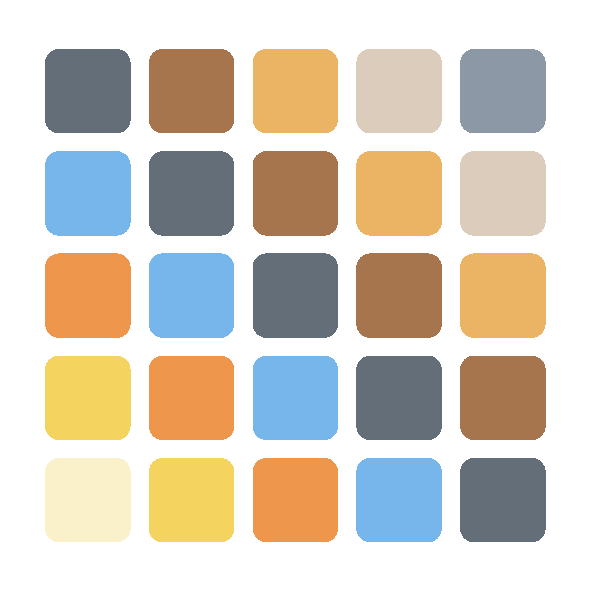
\includegraphics[width=0.65\textwidth]{images/toeplitz_v1.pdf}
      \caption*{}
    \end{subfigure}
    \hfill
    \begin{subfigure}[b]{0.3\textwidth}
      \centering
      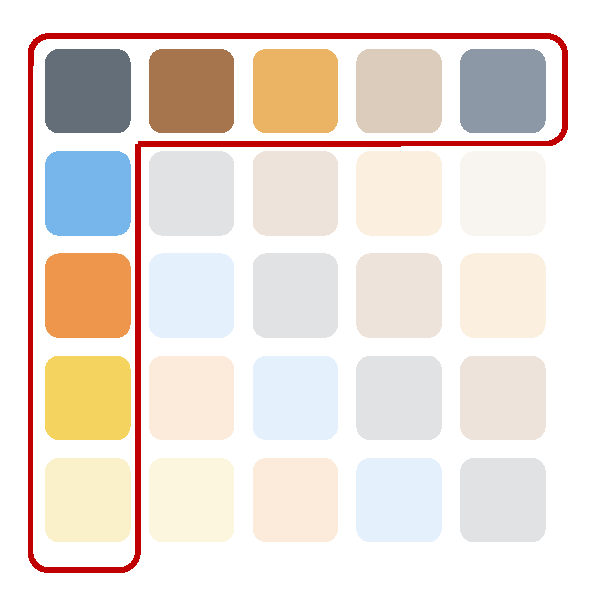
\includegraphics[width=0.65\textwidth]{images/toeplitz_v2.pdf}
      \caption*{}
    \end{subfigure}
  \end{figure}

  $\Rightarrow$ A $n \times n$ Toeplitz matrix has $2n - 1$ unique values. 

  % $\Rightarrow$ We can constraint or generalize the Toeplitz structure.

\end{frame}



%%%%%%%%%%%%%%%%%%%%%%%%%%%%%%%%%%%%%%%%%%%%%%%%%%%%%%%%%%%%%%%%%%%%%%%%%%%%%%%
\begin{frame}{Focus on structured matrices from the Toeplitz family}
%%%%%%%%%%%%%%%%%%%%%%%%%%%%%%%%%%%%%%%%%%%%%%%%%%%%%%%%%%%%%%%%%%%%%%%%%%%%%%%
  
  For our contributions, we study:
  \begin{itemize}
    \item[$\bullet$] Circulant matrices
    \item[$\bullet$] Doubly-block Toeplitz matrices
  \end{itemize}

\end{frame}


%%%%%%%%%%%%%%%%%%%%%%%%%%%%%%%%%%%%%%%%%%%%%%%%%%%%%%%%%%%%%%%%%%%%%%%%%%%%%%%
\begin{frame}{Circulant Matrices}
%%%%%%%%%%%%%%%%%%%%%%%%%%%%%%%%%%%%%%%%%%%%%%%%%%%%%%%%%%%%%%%%%%%%%%%%%%%%%%%

  A $n \times n$ circulant matrix is a matrix where each row is a cyclic right shift of the previous one. 

  % \begin{figure}
  %   \begin{subfigure}[b]{0.3\textwidth}
  %     \centering
  %     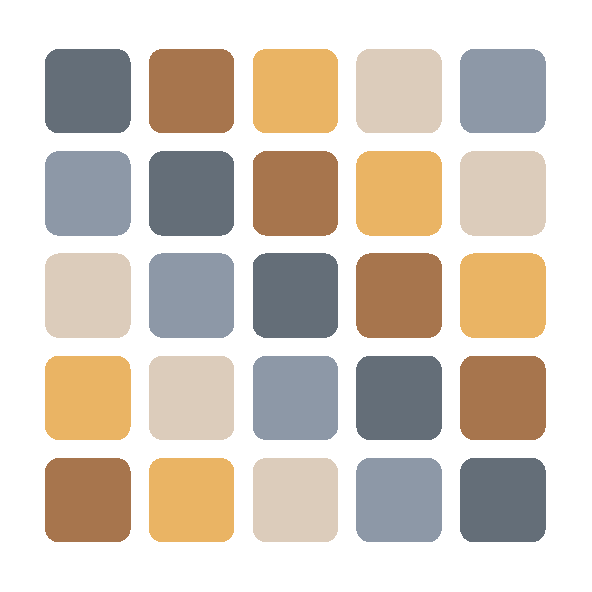
\includegraphics[width=0.65\textwidth]{images/circulant_v1.pdf}
  %     \caption*{A circulant matrix}
  %   \end{subfigure}
  %   \hfill
  %   \begin{subfigure}[b]{0.3\textwidth}
  %     \centering
  %     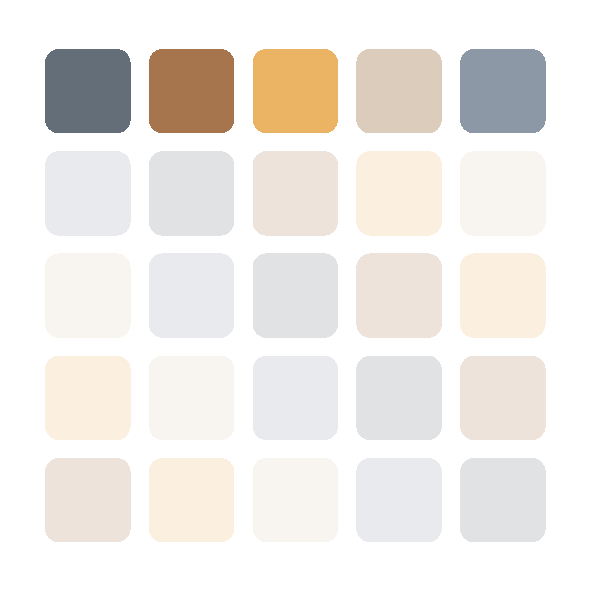
\includegraphics[width=0.65\textwidth]{images/circulant_v2.pdf}
  %     \caption*{First row of a  circulant matrix}
  %   \end{subfigure}
  %   \hfill
  %   \begin{subfigure}[b]{0.3\textwidth}
  %     \centering
  %     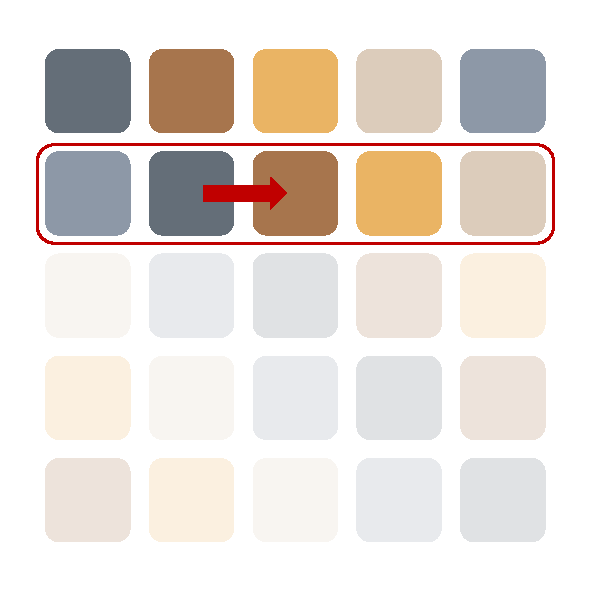
\includegraphics[width=0.65\textwidth]{images/circulant_v3.pdf}
  %     \caption*{First row, shifted on the right}
  %   \end{subfigure}
  % \end{figure}
  
  
  \begin{figure}
    \centering
    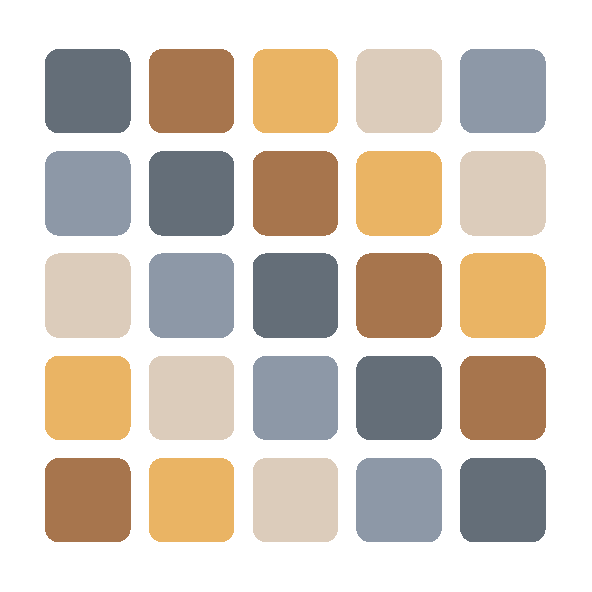
\includegraphics[width=0.35\textwidth]{images/circulant_v1.pdf}
    \caption*{A circulant matrix}
  \end{figure}

\end{frame}


%%%%%%%%%%%%%%%%%%%%%%%%%%%%%%%%%%%%%%%%%%%%%%%%%%%%%%%%%%%%%%%%%%%%%%%%%%%%%%%
\begin{frame}{Doubly-Block Toeplitz Matrices}
%%%%%%%%%%%%%%%%%%%%%%%%%%%%%%%%%%%%%%%%%%%%%%%%%%%%%%%%%%%%%%%%%%%%%%%%%%%%%%%

  A block Toeplitz matrix is a matrix which contains \textbf{blocks that are repeated down the diagonals} of the matrix.

  A \textbf{doubly-block Toeplitz matrix} is a block Toeplitz matrix where all blocks are also Toeplitz.

  \begin{figure}
    \centering
    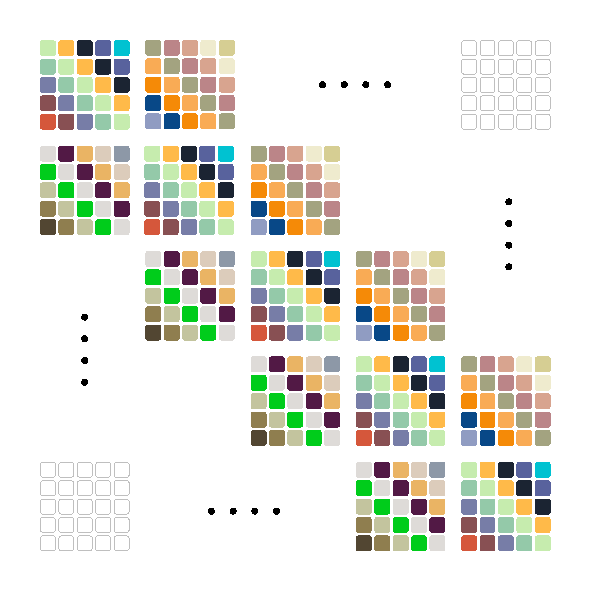
\includegraphics[width=0.35\textwidth]{images/doubly_block.pdf}
    \caption*{Doubly-block Toeplitz matrices}
  \end{figure}

  $\Rightarrow$ Doubly-block matrices are equivalent to the 2d convolution.
  
\end{frame}






% %%%%%%%%%%%%%%%%%%%%%%%%%%%%%%%%%%%%%%%%%%%%%%%%%%%%%%%%%%%%%%%%%%%%%%%%%%%%%%%
% \begin{frame}{Convolutional Neural Networks}
% %%%%%%%%%%%%%%%%%%%%%%%%%%%%%%%%%%%%%%%%%%%%%%%%%%%%%%%%%%%%%%%%%%%%%%%%%%%%%%%
%   Convolutional Neural Networks are state-of-the-art for image classification.
%   \begin{figure}
%     \centering
%     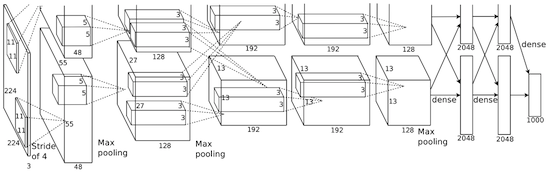
\includegraphics[width=0.8\textwidth]{images/alexnet.png}
%     \caption{Architecture of AlexNet \cite{}}
%   \end{figure}
%   Convolutional Neural Networks use a specific \textbf{structure as linear operations}. 
% \end{frame}


% %%%%%%%%%%%%%%%%%%%%%%%%%%%%%%%%%%%%%%%%%%%%%%%%%%%%%%%%%%%%%%%%%%%%%%%%%%%%%%%
% \begin{frame}{Convolution as matrix-multiplication}
% %%%%%%%%%%%%%%%%%%%%%%%%%%%%%%%%%%%%%%%%%%%%%%%%%%%%%%%%%%%%%%%%%%%%%%%%%%%%%%%
%
%   A discrete convolution between a signal $\xvec$ and a kernel $\kvec$ can be expressed as a product between the vectorization of $\xvec$ and a doubly-block Toeplitz matrix $\Mmat$, whose coefficients have been chosen to match the convolution $\xvec * \kvec$.
%
%   \begin{figure}
%     \begin{subfigure}[t]{0.49\textwidth}
%       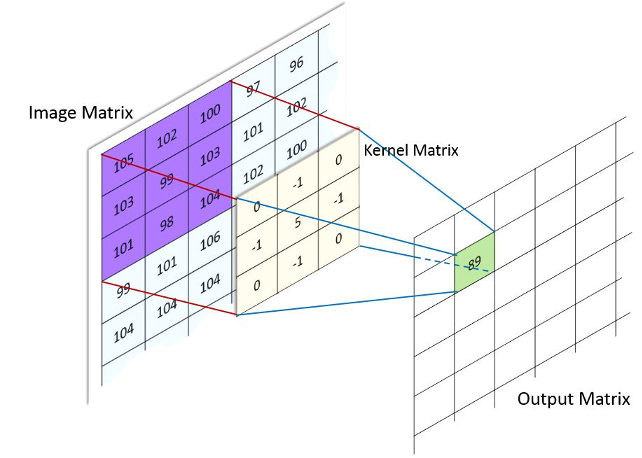
\includegraphics[width=\textwidth]{images/convolution.png}
%       \caption*{Convolution between an 2 dimensional image and a 2 dimensional kernel}
%     \end{subfigure}
%     \begin{subfigure}[t]{0.45\textwidth}
%       \centering
%       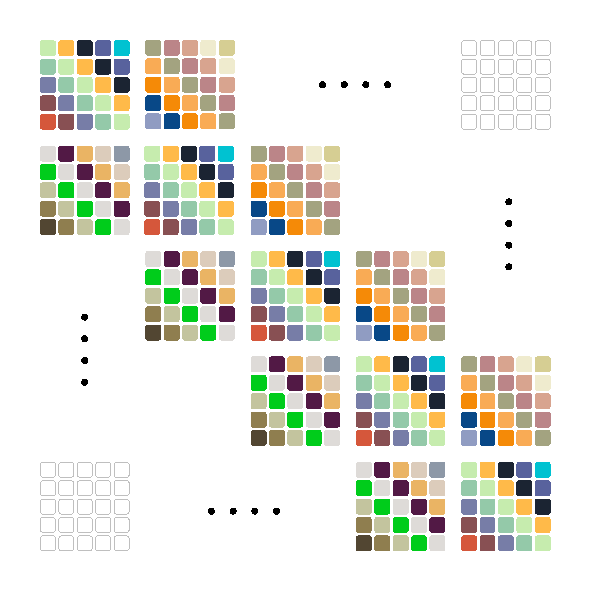
\includegraphics[width=0.8\textwidth]{images/doubly_block.pdf}
%       \caption*{Representation of a Doubly-Block Toeplitz matrix}
%     \end{subfigure}
%   \end{figure}
%
%   When the images has multiples \textit{feature maps}, the matrix $\Mmat$ is the concatenation of multiple Doubly-block Toeplitz matrices.
%   
% \end{frame}


%%%%%%%%%%%%%%%%%%%%%%%%%%%%%%%%%%%%%%%%%%%%%%%%%%%%%%%%%%%%%%%%%%%%%%%%%%%%%%%
\begin{frame}{Our Contributions}
%%%%%%%%%%%%%%%%%%%%%%%%%%%%%%%%%%%%%%%%%%%%%%%%%%%%%%%%%%%%%%%%%%%%%%%%%%%%%%%

  \begin{block}{We devised a compact architecture with Diagonal and Circulant Matrices}
    \begin{itemize}[leftmargin=*]
      \item[] {\small We define the expressive power of diagonal circulant neural networks.}
      \item[] {\small We use diagonal circulant neural networks for compact large scale video classification.}
    \end{itemize}
  \end{block}

  \begin{block}{Improving Robustness of Convolution Neural Networks with Doubly-Block Toeplitz matrices}
    \begin{itemize}[leftmargin=*]
      \item[] {\small We devise an upper bound on the singular values of convolutional layers.}
      \item[] {\small We propose an efficient algorithm to compute this upper bound.}
      \item[] {\small We propose a new regularization scheme to improve the robustness of Neural Networks.}
    \end{itemize}
  \end{block}

\end{frame}



